\section{Crowdsourced-Tracking: Funktionsweise}
\label{sec:Funktionsweise}

Mit der Einführung ihres ersten \ac{BLE}-Trackers hat die Firma Tile 2013 das Konzept eines \ac{BLE}-basierten Tracking-Systems populär gemacht.
Wie viele konkurrierende Systeme, darunter Apples „Wo ist?“ Dienst, setzt auch Tile auf crowdsourcing zur Bestimmung der Position verlorener Gegenstände \cite{Weller_BLE_Finders}.
Die grundlegende Funktion dieser Systeme ist jeweils identisch und in \autoref{fig:tracker_allgemein} gezeigt: Ein zu findendes Gerät \textit{a)} sendet periodisch \ac{BLE}-Advertisements, die von Smartphones in der Nähe \textit{b)}, welche am entsprechenden System teilnehmen, empfangen werden können \textit{(1)}.
Das zu findende Gerät ist dabei entweder ein Endgerät wie ein Smartphone oder ein Tablet, oder ein spezieller, batteriebetriebener, sogenannter Tracker.
Solche Tracker können an anderen Gegenstände befestigt werden, sodass diese bei Verlust ebenfalls gefunden werden können.
Die Empfänger der \ac{BLE}-Advertisements können ihre Position über das \ac{GPS} bestimmen und diese zusammen mit einer ID, welche das zu findende Gerät identifiziert, an einen Server übermitteln \textit{(2)}.
Der Besitzer des verlorenen Geräts \textit{c)} kann die Position seines Geräts vom Server abrufen \textit{(3)} \cite{Garg_Secure_Tracker}.
Das Funktionsprinzip ist dementsprechend vergleichsweise einfach.
\begin{figure}[ht]
    \centering 
    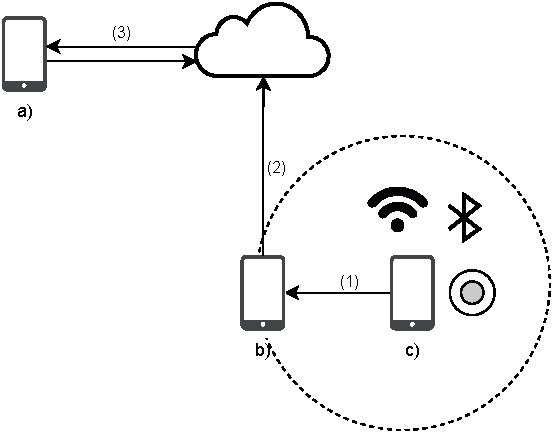
\includegraphics[width=0.9\textwidth]{BLE_Tracker_allgemein.pdf}
    \caption{Allgemeine Funktionsweise des Crowdsourced-Tracking mit \ac{BLE}.}
    \label{fig:tracker_allgemein}
\end{figure}
Qualität und Nützlichkeit für die Nutzer eines solchen Dienstes hängt aber stark von der Anzahl der Nutzer ab.
Die Position eines verlorenen Geräts kann nur vom Tracking-Dienst abgerufen werden, wenn ein Nutzer des gleichen Dienstes ein \ac{BLE}-Advertisement des verlorenen Geräts empfangen und die Position an den Dienst übermittelt hat.
Je mehr Nutzer ein Dienst hat, desto größer die Wahrscheinlichkeit, dass sich ein Nutzer vor kurzem in der Nähe des verlorenen Geräts befand und desto größer die Wahrscheinlichkeit, das verlorene Gerät zu finden.


In allen untersuchten Systemen konnten Weller \textit{et al.} \cite{Weller_BLE_Finders} und Garg \textit{et al.} \cite{Garg_Secure_Tracker} unabhängig voneinander verschiedene Schwachstellen finden, die sowohl Privatsphäre als auch Sicherheit betreffen.
Unter anderem übermittelten einige Dienste die Positionsdaten unverschlüsselt und erlaubten das unberechtigte Abrufen von personenbezogenen Daten über die Backends der Dienste.
Auch zum Veröffentlichungszeitpunkt der Arbeit von Weller \textit{et al.} \cite{Weller_BLE_Finders} waren nicht alle der erkannten Schwachstellen behoben.
Außerdem bot keiner der von Garg \textit{et al.} \cite{Garg_Secure_Tracker} untersuchten Dienste ausreichend Schutz vor dem Melden falscher Positionsdaten.


\subsection{Funktionsweise des „Wo ist?“ Dienstes im Detail}
\label{sec:Funktionsweise_FindMy}
Auf seiner Informationsseite über den „Wo ist?“ Dienst gibt Apple an: „Geräte in der Nähe senden den Standort [...] sicher an iCloud weiter [...]. Zum Schutz der Privatsphäre passiert das alles anonym und verschlüsselt“ \cite{Apple_WoIst}.
Apple erhebt demnach den Anspruch einen Dienst anzubieten, der nicht nur sicherer, sondern auch besser für die Privatsphäre der Nutzer ist als die Dienste der Konkurrenz.
Vergangene Untersuchungen haben allerdings bereits gezeigt, dass auch Apples Dienst einige Schwachstellen aufweist \cite{Heinrich_FindMy,Tonetto_FindMy}.
Diese Schwachstellen werden in \autoref{sec:Missbrauch} wieder aufgegriffen.

Der vermutlich größte Vorteil des Dienstes liegt vermutlich aber in der großen Zahl der Geräte, welche aktiv die Positionsdaten verlorener Geräte sammeln.
Laut Apple nehmen „hunderte[n] Millionen iPhone, iPad und Mac Geräte[n]“ \cite{Apple_WoIst} am „Wo ist?“ Dienst teil.
Der größte Konkurrent Tile hatte im Jahr 2021 laut der bekannten Gadget-Review Webseite \textit{Pocket-Lint} 40 Millionen Nutzer und kann damit für die Lokalisierung auf ein deutlich kleineres Netzwerk zurückgreifen als Apple \cite{Tile_Network}.


Auf Basis des Reverse-Engineering des „Wo ist?“ Dienstes von Heinrich \textit{et al.} in \cite{Heinrich_FindMy} und der Spezifikation für Drittanbieter \cite{Apple_FindMySpec} wird im Folgenden die grundlegende Funktionsweise des Dienstes erläutert.
Dabei wird insbesondere darauf eingegangen, welche Maßnahmen Apple ergreift um Sicherheit und Privatsphäre der Nutzer besser zu schützen als die konkurrierenden Dienste. 

In der Spezifikation werden folgende vier Rollen definiert \cite{Apple_FindMySpec}:
\begin{itemize}
    \item \textbf{Owner Device}: Alle Geräte, in denen die Apple-ID des Besitzers hinterlegt ist.
    \item \textbf{Accessory}: Das zu findende Gerät.
    \item \textbf{Find My network}: Die Menge aller Apple-Geräte, mit aktivierter „Wo ist?“ Funktion. Einzelne Geräte werden jeweils als \textbf{Finder Device} bezeichnet.
    \item \textbf{Apple Server}: Server der die Standortinformationen speichert.
\end{itemize}
\autoref{fig:findMy_roles} zeigt die Rollen, deren Beziehungen und die jeweiligen Aufgaben wie in der Spezifikation angegeben.
\begin{figure}
    \centering
    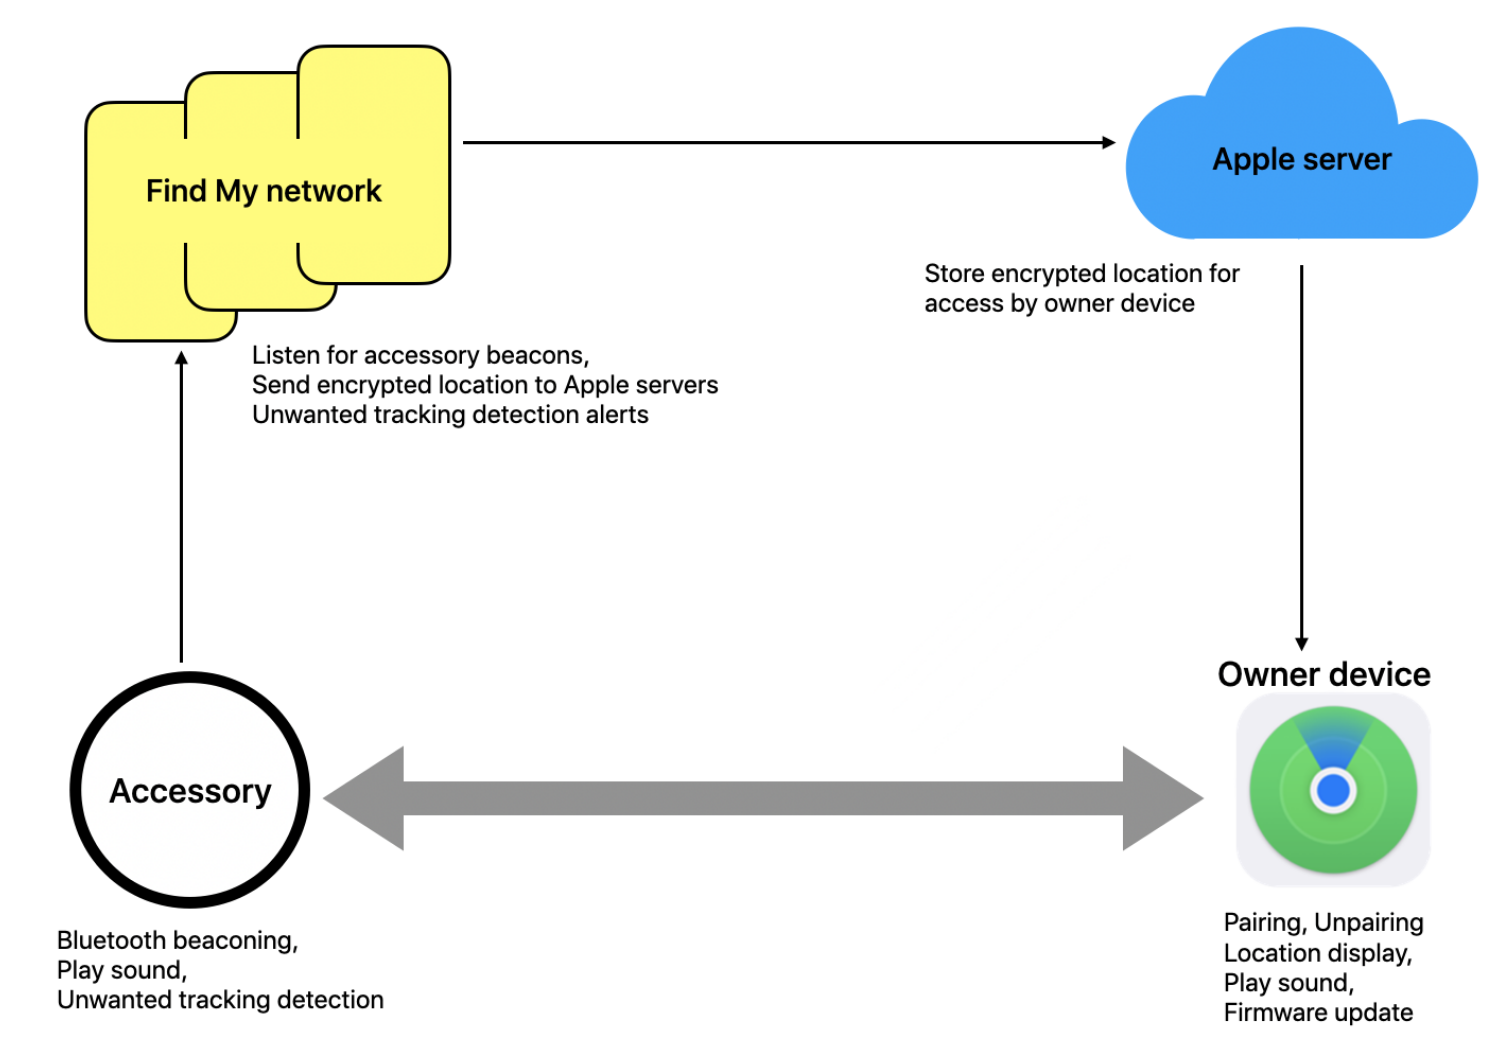
\includegraphics[width=0.9\textwidth]{findMy_roles}
    \caption{Rollen im „Wo ist?“ Dienst \cite{Apple_FindMySpec}.}
    \label{fig:findMy_roles}
\end{figure}
Apple erlaubt seit April 2021 auch Drittanbietern die Nutzung des „Wo ist?“ Netzwerks um die eigenen Produkte zu finden \cite{Apple_FindMy3rdParty}.
Da die Spezifikation speziell für Drittanbieter erstellt wurde, wird das zu findende Gerät als \textit{Accessory} bezeichnet.
In der folgenden Beschreibung wird jedoch der Begriff \textit{Lost Device} verwendet, der auch von Heinrich \textit{et al.} \cite{Heinrich_FindMy} verwendet wird und sowohl Produkte von Drittanbietern als auch von Apple abdeckt.
Das zu findende Gerät muss mit der Apple-ID des Besitzers verbunden sein, um gefunden werden zu können.
Drittanbieter Geräte und AirTags müssen dazu vor der ersten Verwendung über einen Pairing-Prozess mit einem Apple-Gerät verbunden werden \cite{Apple_FindMySpec}.

\subsubsection{Kryptografie}
\label{sec:Kryptografie}

Um bessere Sicherheit und Privatsphäre als die Konkurrenz zu bieten, setzt Apple auf asymmetrische \ac{ECC} Verschlüsselung.
Standortdaten werden immer Ende-zu-Ende verschlüsselt, sodass potenzielle Angreifer die Positionen der Nutzer nicht verfolgen können, sollten sie an Standortdaten gelangen.
Durch den verwendeten Prozess zur Verschlüsselung kann auch Apple selbst nicht auf die Standortdaten zugreifen.
Nur der Besitzer des Geräts kann die Standortdaten zur Lokalisierung des Geräts entschlüsseln \cite{Greenberg_FindMyCrypto}.


Jedes Owner Device erstellt zunächst den sogenannten \textit{Master Beacon Key}, bestehend aus einem \ac{ECC} Schlüsselpaar und einem symmetrischen Schlüssel.
Diese Schlüssel werden über den iCloud Dienst zwischen allen Geräten mit der gleichen Apple-ID synchronisiert.
Um die Schlüssel bei der Synchronisierung zu schützen, werden sie mit einem symmetrischen Schlüssel, aus der als sicher geltenden iCloud Keychain, verschlüsselt \cite{Heinrich_FindMy,Afonin_iCloudKeychain}.
Der private Schlüssel des \ac{ECC}-Schlüssels sowie der symmetrische Schlüssel des Master Beacon Keys müssen geheim bleiben.
Auch der öffentliche Teil des \ac{ECC}-Schlüssels im Master Beacon Key, wird nie über \ac{BLE} übertragen.
Stattdessen wird der Master Beacon Key verwendet, um temporär gültige Schlüssel abzuleiten, die im \ac{BLE}-Advertising übertragen werden können.
Für die Ableitung dieser sogenannten \textit{Advertising Keys} wird die ANSI X9.63-\ac{KDF} verwendet \cite{Apple_FindMySpec}.
Aus einem im \ac{BLE}-Advertising übertragenen öffentlichen Schlüssel kann somit, ohne Kenntnis des Master Beacon Keys, der nächste öffentliche Schlüssel nicht abgeleitet werden.
Durch regelmäßiges Wechseln des verwendeten Avertising Keys wird es einem Angreifer erschwert, ein Lost Device anhand der im Advertising übertragenen Daten zu verfolgen.
Da für die Verschlüsselung der Standortdaten nur die X-Koordinate des öffentlichen Schlüssels benötigt wird, kann auf die Übertragung der Y-Koordinate verzichtet werden \cite{Heinrich_FindMy}.

Die Verschlüsselung der Standortdaten erfolgt auf dem Finder Device mit dem \ac{AES}-Algorithmus im \ac{GCM}-Modus.
Aus dem, vom Finder Device empfangenen, Advertising Key wird ein temporäres \ac{ECC}-Schlüsselpaar generiert, aus welchem über einen \ac{ECDH} Schlüsselaustauch ein geteiltes Geheimnis generiert und durch die Anwendung der ANSI X9.63-\ac{KDF} ein symmetrischer Schlüssel abgeleitet wird.
Der Schlüsselaustausch verwendet den privaten Teil des temporären \ac{ECC}-Schlüssels und den öffentlichen Teil des empfangenen Advertising Keys.
Von diesem werden die ersten 16 Byte als Schlüssel für den \ac{AES}-Algorithmus und die folgenden 16 Byte als Initialisierungsvektor verwendet \cite{Heinrich_FindMy}.
Durch die Ausführung der Verschlüsselung auf dem Finder Device, kann die Batterie des Lost Devices geschont werden und die Lokalisierung verlorener Geräte bleibt länger möglich.
Insbesondere bei AirTags oder Produkten von Drittanbietern kann das hilfreich sein, da diese Geräte, eine im Vergleich zu einem iPhone oder iPad, sehr geringe Batteriekapazität haben.
Die kryptografischen Funktionen könnten den Stromverbrauch der Geräte deutlich erhöhen, wenn bei jedem Kontakt mit einem Finder-Device dieser komplexe Verschlüsselungsprozess ablaufen muss.
Durch die Verschlüsselung auf den Finder Devices müssen die Lost Devices nur alle 15 Minuten einen neuen Schlüssel ableiten, was durch die geringere Zahl der Operationen eine deutlich geringere Belastung für die Batterie darstellt.


Für die Entschlüsselung kann das geteilte Geheimnis über den \ac{ECDH} Schlüsselaustausch mit dem öffentlichen Teil des temporären Schlüssels und dem privaten Teil des Advertising Keys berechnet werden.
Der symmetrische Schlüssel entsteht wieder durch die Anwendung der ANSI X9.63-\ac{KDF} auf das geteilte Geheimnis.
Damit ist sichergestellt, dass die verschlüsselten Daten nur vom Besitzer entschlüsselt werden können.
Dieser kann die für das Advertisement verwendeten Schlüsselpaare unabhängig vom verlorenen Gerät aus dem Master Beacon Key ableiten und hat somit Zugriff auf die privaten Schlüssel.
Der öffentliche Teil des temporären Schlüssels und ein \ac{SHA}-256 Hash des verwendeten Advertisement Keys wird mit den verschlüsselten Daten auf Apples Server hochgeladen.
Der Besitzer kann diese Daten abrufen und aus der Kombination des öffentlichen temporären Schlüssels und dem privaten Advertisement Keys das geteilte Geheimnis und somit den symmetrischen Schlüssel berechnen \cite{Heinrich_FindMy}.

Da Geräte ohne Internetverbindung, wie zum Beispiel AirTags oder andere Geräte von Drittanbietern, die Master Beacon Keys nicht über die iCloud Synchronisation erhalten können, müssen diese Geräte auf andere Weise an einen initialen Schlüssel kommen.
% TODO: Schlüsselaushandlung, Infos aus Spec

\subsubsection{Ablauf beim Verlust eines Geräts}
\label{sec:Verlust}

Alle Apple Geräte mit aktivierter Bluetooth-Funktion, die für das Finden durch den „Wo ist?“ Dienst angemeldet sind, senden periodisch, in der Regel im Advertising Intervall von 2 s \ac{BLE}-Advertisements.
Die im Advertisement enthaltenen Daten unterscheiden sich jedoch abhängig vom Zustand des Geräts.
iPhones, iPads und MacBooks mit Internetverbindung und alle unterstützen Geräte mit einer aktiven \ac{BLE}-Verbindung mit einem Owner Device, gelten nicht als Lost Device und senden deshalb nur die ersten fünf Bytes des öffentlichen Advertisement Keys.
Das Advertisement erfolgt vermutlich um erkennen zu können, wenn ein Gerät in der Nähe die Verbindung verliert.
Die ersten fünf Byte des öffentlichen Schlüssels sollten in der Regel ausreichen um verschiedene Geräte voneinander unterscheiden zu können.
Vermutlich werden Funktionen, wie die Warnung beim Zurücklassen eines Geräts \cite{Apple_FindMyWarning}, über diese Advertisement Daten umgesetzt.

Sobald ein Gerät die Internetverbindung oder die \ac{BLE}-Verbindung zum Owner Device verliert, wird es als Lost Device angesehen.
Um in diesem Zustand von anderen Finder Devices gefunden zu werden, beginnt das Lost Device \ac{BLE}-Advertisements mit dem kompletten öffentlichen Advertisement Key zu senden \cite{Apple_FindMySpec}.
Die Advertisement Pakete werden immer mit dem Typ \textit{manufacturer-specific data} gesendet, sodass neben angebotenen \ac{BLE}-Services auch eigene Daten übertragen werden können.
Das Format erlaubt nach einer Firmen-ID von zwei Byte, maximal 27 weitere Byte zu übertragen.
Da Apple, die manufacturer-specific data auch für andere Zwecke, wie zum Beispiel AirDrop nutzt, wird jeweils ein weiteres Byte für den Typ ($0x12$) des Pakets und dessen Länge verwendet.
Zur Identifikation des Lost Device und zur Verschlüsselung der Standortdaten müssen die 28 Byte der X-Koordinate des aktuellen öffentlichen Schlüssels im Advertisement übertragen werden \cite{Heinrich_FindMy}.
Jeder Schlüssel wird für 15 Minuten verwendet, um die Verfolgung des Geräts anhand der Advertising-Daten für Dritte zu erschweren.
Nach Ablauf der 15 Minuten wird ein neuer Schlüssel abgeleitet und für die nächste Periode im Advertisement versendet.
Da der Schlüssel aus dem Advertising alleine nicht reicht, um den nächsten Schlüssel abzuleiten, kann so die Privatsphäre im Vergleich zu Konkurrenzprodukten verbessert werden.
Die 25 Byte Payload reichen nicht aus, um die X-Koordinate des öffentlichen Schlüssels zu übertragen.
Deshalb  wird zusätzlich die Advertising Address des Advertisement Pakets ausgenutzt.
Die Advertising Address kann zum Schutz der Privatsphäre laut \ac{BLE}-Spezifikation \cite{Spec_BLE_5.3} von der tatsächlichen \ac{MAC}-Adresse des Geräts abweichen.
Üblicherweise wird diese Funktion verwendet um über zufällige \ac{MAC}-Adressen die Nachverfolgbarkeit von Geräten und Rückschlüsse auf den Gerätehersteller zu erschweren.
Durch Codierung von Daten in der zufälligen Adresse, kann das Feld jedoch für den Transfer beliebiger Daten ausgenutzt werden.
Apple speichert die ersten 46 Bit des öffentlichen Schlüssels in der Advertising Address, wobei die beiden \acp{MSB} des ersten Bytes jeweils auf 1 gesetzt werden müssen, um der \ac{BLE}-Spezifikation zu genügen \cite{Heinrich_FindMy}.
Die restlichen 170 Bit bestehend aus den Bytes 6 bis 27 und den fehlenden zwei Bits des Byte 0 werden im Advertising Payload übertragen \cite{Apple_FindMySpec}.
\autoref{fig:apple_advertising} zeigt den resultierenden Aufbau eines Advertisement Pakets des „Wo ist?“ Dienstes.
Die Teile, in welchen der öffentliche Schlüssel übertragen wird, sind gelb hinterlegt.
Das als "Hint" bezeichnete Feld codiert laut Spezifikation \cite{Apple_FindMySpec} Byte 5 des öffentlichen Schlüssels, laut Heinrich \textit{et al.} \cite{Heinrich_FindMy} ist dieses Feld bei iOS immer 0.
Mit einem eigenen \ac{BLE}-Scan konnte beobachtet werden, dass das Feld bei einem iOS-Gerät auf 0 gesetzt war, obwohl Byte 5 des öffentlichen Schlüssels ungleich 0 war.
Dementsprechend wird dieses Byte vermutlich nur bei Drittanbieter-Produkten und eventuell bei AirTags verwendet.
% TODO: test mit Airtag?
\begin{figure}
    \centering
    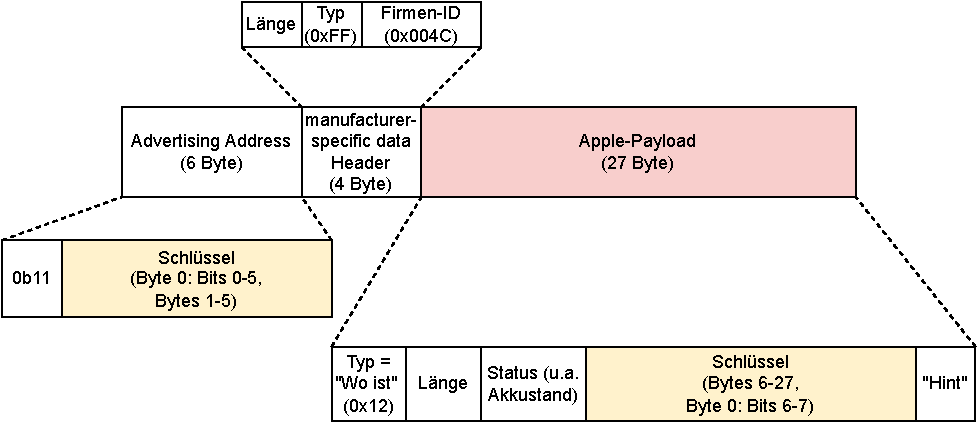
\includegraphics[width=0.9\textwidth]{apple_advertising.pdf}
    \caption{Aufbau der Advertisement Pakete des „Wo ist?“ Dienstes.}
    \label{fig:apple_advertising}
\end{figure}

Standardmäßig scannen alle Apple-Geräte (Finder-Devices) im Hintergrund nach Advertisements, die die Firmen-ID von Apple enthalten.
Wird ein Paket durch den Apple Payload Typ $0x12$ als Advertisement für den „Wo ist?“ Dienst identifiziert, wird vom Finder Device zunächst die aktuelle Position bestimmt und ein sogenannter \textit{Location Report} erstellt.
Das Format dieses Reports ist in \autoref{fig:location_report} gezeigt.
\begin{figure}
    \centering
    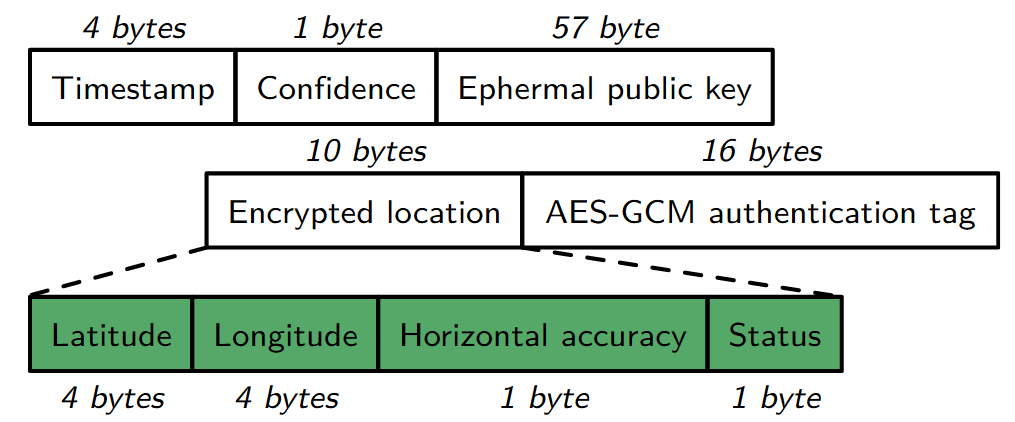
\includegraphics[width=0.85\textwidth]{location_report}
    \caption{Format des Location Reports \cite{Heinrich_FindMy}}
    \label{fig:location_report}
\end{figure}
Der Hauptbestandteil des Reports sind die wie oben beschrieben verschlüsselten Standortinformationen, bestehend aus Koordinaten, Genauigkeit und Status.
Außerdem sind sowohl der temporäre Schlüssel, welcher vom Finder-Device aus dem Advertisement Key abgeleitet und für den \ac{ECDH}-Schlüsselaustausch genutzt wurde, und der \ac{AES}-\ac{GCM} Authentication Tag teil des Reports.
Daneben findet sich unter anderem der Zeitstempel zum Zeitpunkt der Erstellung des Reports.
Beim Upload wird der Report mit einem \ac{SHA}-256 Hash des verwendeten Advertisement Keys verknüpft, um die Identifizierung zu ermöglichen \cite{Heinrich_FindMy}.
Im Vergleich zu konkurrierenden Diensten ist die Verschlüsselung ein wichtiger Schritt, um die Sicherheit und Privatsphäre des Dienstes zu verbessern.
Meist werden Reports nicht unmittelbar nach der Erstellung hochgeladen.
Stattdessen sammelt das Gerät mehrere Reports und lädt diese gebündelt hoch.
Der empfangende Server ordnet den Reports zusätzlich den Zeitstempel zum Zeitpunkt des Datenempfangs zu.
Tonetto \textit{et al.} \cite{Tonetto_FindMy} haben gezeigt, dass die Art der Internetverbindung beeinflusst, wann die Reports hochgeladen werden.
So liegt der Median für den Upload eines Reports bei aktiver WLAN-Verbindung bei 15 Minuten während bei aktiver Mobilfunkverbindung der Median bei 3 Stunden liegt.
Der Upload erfolgt über einen HTTPS-Request, der zusätzlich über den Header authentifiziert wird.
Dieser Header enthält unter anderem ein Identitäts-Zertifikat des Geräts und eine Signatur des Requests.
Diese Signatur wird mit dem privaten Schlüssel erstellt, welcher in einem speziellen Sicherheitsbereich, dem \textit{Secure Enclave Processor} des Geräts gespeichert ist, welcher das unberechtigte Auslesen verhindert.
Somit kann vermutlich sichergestellt werden, dass nur Apple Geräte in der Lage sind Reports hochzuladen, was das Erstellen gefälschter Reports erschwert \cite{Heinrich_FindMy}.


Um die Standortdaten vom Server abzurufen, wird ein über Basic Authentication mit der Apple-ID des Nutzers und einem Token authentifizierter, HTTPS-Request verwendet.
Die Anfrage enthält zusätzlich eine Liste der letzten Advertisement Keys des verlorenen Geräts.
So können die verschlüsselten Location Reports heruntergeladen und anschließend auf dem Gerät entschlüsselt werden, um das verlorene Gerät zu lokalisieren \cite{Heinrich_FindMy}.
\autoref{lst:findmy_result} zeigt die Struktur der Antwort auf einen solchen Request in gekürzter Form.
Die Antwort besteht aus einem Array von Objekten, die jeweils den Hash des Advertisement Keys, einen verschlüsselten Location Report und Metadaten, darunter den Zeitstempel des Datenempfangs, enthalten.
Anhand des Hashes kann der für die Entschlüsselung zu verwendende Advertising Key bestimmt werden.
Entschlüsselte Standortdaten aus mehreren Reports können kombiniert werden, um Genauigkeit bei der Positionsermittlung zu erhöhen.
Gleichzeitig können die Daten mehrerer Reports auch dazu verwendet werden, den Pfad des verlorenen Geräts zu rekonstruieren.
Dafür können bis zu sieben Tage alte Positionen vom Server abgerufen werden \cite{Heinrich_FindMy}.

\begin{lstlisting}[label=lst:findmy_result,caption={Beispielhafte Antwort beim herunterladen von Location Reports\cite{Heinrich_FindMy}.}]
{
    "results": 
    [
        {
            "datePublished": 1586804587284,
            "payload": "JETtmwIEzRBG ....",
            "description": "found",
            "id": "B6E5tpUPbuudAc ...",
            "statusCode": 0
        },
        ...
    ] ,
    "statusCode": "200"
}
\end{lstlisting}